\documentclass[aspectratio=169]{beamer}

\usepackage[utf8]{inputenc}
\usepackage[brazil]{babel}
\usepackage{graphicx}
\usepackage{hyperref}
\usepackage{amssymb}

% Tema simples e limpo
\usetheme{Madrid}
\usecolortheme{default}
\setbeamertemplate{navigation symbols}{}

% -------------------------------------------------
% INFORMAÇÕES DO EP (OS ALUNOS DEVEM EDITAR)
% -------------------------------------------------

\title{MAC0209 --- Modelagem e Simulação}
\subtitle{Exercício-Programa 1 --- \textit{Floats} e Precisão}
\author[Grupo Plutão]{Grupo Plutão \\[4pt]
Guilherme França Carvalho \\
Ismália Alves Santos Ziemer \\
João Victor Bispo do Nascimento \\
Leonardo Heidi Almeida Murakami \\
Luis Renato Ferraz Natil Martins \\
Murilo Freitas Yonashiro Coelho \\
Vítor Gonçalves Serra \\
Vitor Wallace de Moraes Alves }
\institute[BCC IME-USP]{Bacharelado em Ciência da Computação \\ IME -- USP}
\date{\today}

% -------------------------------------------------

\begin{document}

% =================================================
% SLIDE 1
% =================================================
\begin{frame}
\titlepage
\end{frame}

\begin{frame}{Contexto e Objetivo do EP}

\textbf{Contexto do curso}

\begin{itemize}
    \item Dados são discretizados quando processados pelo computador
    \begin{itemize}
        \item Não é possível calcular no contínuo - processo de amostragem
            \begin{equation}
                x[n] = x(n\Delta t), n \in \mathbb{Z}
            \end{equation}
        \item Resultados e parâmetros são arrendondados - processo de quantização
            \begin{equation}
                \overline x[n] = Q(x[n]) \quad \text{(Q tem saída discreta)}
            \end{equation}
    \end{itemize}
    \item Laboratório: Exemplos com funções seno, log, arcotangente
\end{itemize}

\vspace{0.5cm}

\textbf{Objetivo do EP}

\begin{itemize}
    \item Entender \textbf{problema inverso}, determinar paramêtros
        desconhecidos a partir de observações do fenômeno
    \item Comparar os métodos analítico e numérico para solucionar uma EDO (equação diferencial ordinária)
    \item Entender como os dados são discretizados (amostragem e quantização)
\end{itemize}

\end{frame}

% =================================================
% SLIDE 2
% =================================================
\begin{frame}{Trabalho Realizado}

\textbf{Conceitos e implementação}

\begin{itemize}
    \item Método analítico: integração da EDO para obter a função da posição
        $x(t)$
    \item Método de Euler: uso de um sistema de $N$ EDOs para solucionar uma EDO
        de ordem $N$, equações da forma $x(t + \Delta t) = x(t) + \Delta t
        \frac{dx(t)}{dt}$ para $\Delta t$ suficientemente pequeno
    \item Implementação dos métodos analítico e numérico de Euler para solucionar uma EDO
    \item Escolha dos parâmetros $a=2, v_0=-1, x_0=0, \Delta t=0.01$

\end{itemize}

\end{frame}

% =================================================
% SLIDE 3
% =================================================
\begin{frame}{Resultados e Conclusões}

\textbf{Resultados}

\begin{itemize}
    \item O erro, diferença entre o resultado dos métodos analítico e de Euler,
        diminui conforme $\Delta t$ diminui. Mas para $\Delta t$ muito pequeno 
        surgem erros de floating point que diminuem a precisão do cálculo
    \item Para calcular $x(t)$ pelo método de Euler, é necessário calcular os
        resultados sequencialmente, enquanto pelo método analítico podemos
        calcular $x(t)$ diretamente
    \begin{figure}[b]
        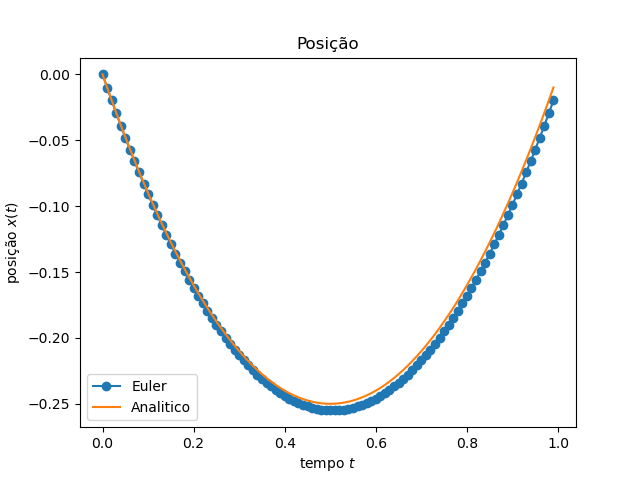
\includegraphics[width=4cm]{images/plot_pos.png}
        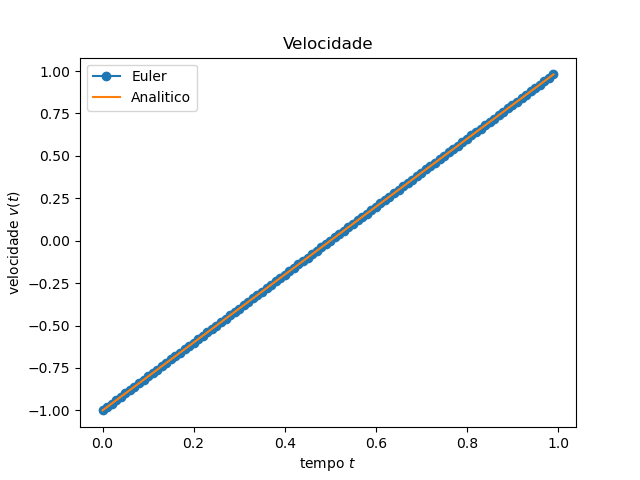
\includegraphics[width=4cm]{images/plot_vel.png}
        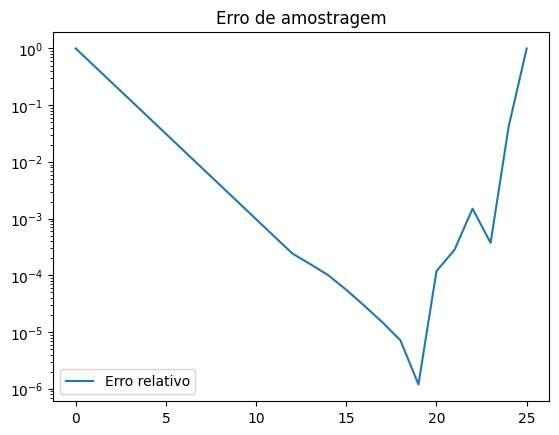
\includegraphics[width=4cm]{images/plot_erro-de-amostragem.jpeg}
        \caption{$a=2, v_0=-1, x_0=0, \Delta t=0.01 \quad\quad \Delta t = 2^{-k}, k \in \mathbb{N}, k = [0; 26]$}
    \end{figure}

\end{itemize}

\end{frame}

\end{document}
